\documentclass{scrartcl}
\usepackage[utf8]{inputenc}
\usepackage[T1]{fontenc}

\usepackage[american]{babel}
\usepackage[autostyle, english = american]{csquotes}
 \usepackage[maxbibnames=10,
   backend=biber]{biblatex}
 \addbibresource{../bibliography.bib}

\usepackage[final,tracking=smallcaps,expansion=alltext, protrusion=true]{microtype}
\SetTracking{encoding=*, shape=sc}{50} %latex & friends, page 52
\usepackage{todonotes}
\usepackage{caption}
\usepackage{booktabs}
\usepackage{siunitx}
\usepackage{etoolbox}

\newrobustcmd*{\bftabnum}{%
  \bfseries
  \sisetup{output-decimal-marker={\textmd{.}}}%
}
\sisetup{detect-weight=true,detect-inline-weight=math}


\usepackage{float}
\usepackage{subcaption}
\usepackage{bm}
\usepackage{amsmath}
\usepackage{amsfonts}
\usepackage{amssymb}
\usepackage{nicefrac}
\usepackage{mathtools} % for \mathclap
\usepackage{hyperref}
\usepackage[noabbrev]{cleveref}
\newcommand{\creflastconjunction}{, and\nobreakspace} % use Oxford comma
%\usepackage{placeins} % for floatbarrier

\usepackage{tikz}
\usetikzlibrary{arrows, positioning, shapes.geometric}
\usetikzlibrary{calc}
\graphicspath{{../../figures/}}

\newcommand{\img}{\bm{f}} % TODO: Format

\begin{document}
\title{Deep-Learning-based Image Denoising in Ophthalmology}
\author{Lukas Krenz}

\maketitle

\section{Introduction}
Intraoperative medical imaging is an important part of modern surgery.
This project is focussed mostly on the example of retinal membrane peeling, which is an ophthalmic operation.
While high quality images are available in the diagnostic phase, this is not true during operations.

During ophthalmic procedures, the surgeon manipulates anatomical structures of the retina with micron-scale maneuvers while observing the scene indirectly via microscope.
The resulting magnification has the effect that only a small area is focussed, other parts are either distorted or occluded.
Additionally, the motion of the eye introduces blur.
All these factors result in images which are corrupted by noise.
This makes precise operations more difficult.
The intraoperative images not only differ from the diagnostic ones in terms of quality.
During surgery, instruments are present and the membrane is stained with a coloring agent to amplify its edges.

Our goal is to increase the resolution of retinal fundus images both for diagnostic and intraoperative images.
Assuming that we have a measured image \(\hat{\img}\) that is downsampled by an unknown operator \(\operatorname{\downarrow}\),
\begin{equation}
  \label{eq:model}
  \hat{\img} = \operatorname{\downarrow}(\img),
\end{equation}
the goal is to find the best reconstruction of the original image \(\img\).
We consider two different models for \(\operatorname{\downarrow}\):
\begin{itemize}
\item Downsampling by decresead spatial resolution.
  In our case we want to reconstruct an image that was downscaled by a factor of $4$.
  In the literature, this problem is called single image super resolution.
\item Downsampling by decreased sharpness.
  For this case we try to increase the quality of images by removing blur.
\end{itemize}

An image restoration algorithm has to fulfil the following requirements to be considered useful in an intraoperative setting:
\begin{enumerate}
\item All processing should happen in real time.
\item It has to work with images of varying quality, level of zoom and different positions of surgical instruments.
\item The anatomical structure, the position of surgical instruments, and the color have to be conserved.
Both blood vessels and the border of the membrane should be at least as clearly visible as in the original images.
This implies that we have to preserve the image edges.
\end{enumerate}
These constraints can be fulfilled by a deep learning approach.

During the last few years a vast amount of different neural network topologies has been published.
Most of them work on a larger amount of data than we have available and are complex models that do not work in real-time.
The goal of this guided research is to compare different approaches for the denoising and upscaling of the aforementioned pictures.
The main challenge of this project is finding a good trade-off between the resulting image quality and the usability during surgery.

We make the following contributions:
\begin{enumerate}
\item We compare different loss functions and their suitability for medical image denoising.
\item We present models that are able to reconstruct images detoriated by both mentioned downsampling operators in real-time.
\item We evaluate the resulting algorithms on both diagnostic and intraoperative images and discuss their robustness against Blur.
  This is combined with a discussion of the effectiveness of our transfer learning approach.
\end{enumerate}

% \section{Literature Review}
% \subsection{Architectures}
% \label{sec:architecturs}
% Differentiate between methods optimised for quality and speed.
% Quality mostly feeds in a upsampled image, filters for in HR-space.
% Efficiency uses low-resolution image as input, upscales at end.

% We are mostly interested in networks that use a structure that is optimized for efficiency.
% All these structures (or at least the cited examples) have one thing in common:
% They use the low-resolution image as input.
% \begin{description}
% \item[Laplacian Pyramid] Structure used by~\cite{LapSRN}.
%   Progressive upsampling, predict subband residual for each upsampling step.
%   Feature extraction at \textit{coarse}, not \textit{fine} level.
%   Same network can do upsampling at different scales.
%   Uses deep supervision, each resulting image contributes to the loss.
% \item[Hourglass] Used for example by~\cite{Fsrcnn}.
%   Structure of form (Feature extraction -> Shrinking -> Mapping -> Expanding -> Deconvolution).
%   The filters (except deconvolution) are similar for different upscaling factors, makes retraining easy.
% \item[Subpixel Convolution]  Used by~\cite{Espcn}.
%   $L$ convolution layers for feature maps, one subpixel convolution layer with $L$ filters.
%   In~\cite{Espcn} $L = 3$.
% \end{description}

% The following architectures/papers are optimised for quality without regarding the run-time:
% \begin{description}
% \item[Residual Blocks] Used for example by~\cite{EnhanceNet, SRGAN, EDSR}.
%    In case of \textbf{EnhanceNet}: structure of form (Conv -> Residual* -> (NNUpsampling -> Conv)* -> Conv) with 10 residual blocks.
  
% \item[Deeply Recursive] Used by~\cite{DRCN}.
%   Extremely expensive to train (6 days on Titan X).
%   Training relies on several tricks.
%   Structure of (embedding network -> recursive inference network -> reconstruction network)
% \end{description}

% More architectures are discussed in the paper~\cite{NTIRE2017} which describes a contest that was won by~\cite{EDSR}.
% Most approaches used in this challenge are not real-time capable.

% \subsection{Loss functions}
% \label{sec:loss}

% \begin{description}
% \item[MSE] Standard pixelwise mse, optimizes PSNR, leads to blurry images
% \item[Charbonnier-Loss] Pixelwise (differentiable approximation of) $L_1$ error, is more robust, used by~\cite{LapSRN}.
%   Defined typically as
%   \begin{align}
%     \label{eq:charbonnier}
%     L( \hat{\bm{y}}, \bm{y}; \bm{\theta}) = \sum_n p \left( \bm{\hat{y}} - \bm{y} \right)
%     \intertext{with }
%     p(\bm{x}) = \sqrt{ \langle x, x \rangle  + \epsilon^2},
%   \end{align}
%   where $\varepsilon$ is a parameter.
% \item[Perceptual Loss] Don't compare pixel-wise but consider difference of filtered images.
%   Can be defined for an arbitrary filter map as
%   \begin{equation}
%     \label{eq:perceptual-loss}
%    L_p = \Vert \phi( \bm{\hat{y}} ) - \phi (\bm{y}) \Vert_2^2 .
%   \end{equation}
%   The filter maps $\phi$ are often taken from the pooling layers of the VGG-19 network, e.g. EnhanceNet uses the second and fifth~\cite{EnhanceNet}.
%   Leads to visually better images but decreased PSNR.
%   See~\cite{PerceptualLoss} for motivation/details.
% \item[Saliency Loss] The same as the perceptual loss but with handcrafted filters.
%   One example for this is~\cite{SaliencyGAN} which uses the curvature of the image, distribution of elements in a neighborhood and uniqueness of feature maps.
%   This loss is handcrafted for vessel-detection.
% \item[Texture Loss] Use patch-wise correlations of perceptive loss, similar to style transfer. See~\cite{EnhanceNet}.
% \item[Adversarial Loss] Optimize linear combination of other loss and loss function learned by discriminator/critic network.
%   Leads to visually pleasing images, reduced PSNR and might lead to ``imagined'' artifacts.
%   First seen in~\cite{SRGAN}.
%   Mostly classical GAN architectures are used, might make sense to explore more recent variants for easier training (e.g.\ WGAN-GP).
  
% \end{description}
% \subsection{Evaluation}\label{sec:evaluation}
% \begin{description}
% \item[PSNR] Peak-Signal-To-Noise-Ratio. Scaled version of \textsc{mse}, higher values correspond to lower error, defined by:
%   \begin{equation}
%   \label{eq:psnr}
%   \mathrm{PSNR} = -10 \log_{10} (\mathrm{MSE}).
% \end{equation}
% \item[SSIM] Structural similarity index. Tries to measure perceived quality of images.
% \end{description}

% Either use metrics such as PSNR/SSIM, compare visually, or use efficiency as pre-processing, e.g. improved segmentation results

% \subsection{Relevant results}
% Difficult to compare, visual quality does not correspond directly to improved error!
% For \textsc{psnr}-results see~\cref{tab:results}.

% \begin{table}[]
% \centering
% \caption{Some Results, all measured in \textsc{psnr}}

% \label{tab:results}
% \begin{tabular}{@{}llll@{}}
% \toprule
% Model          & SET5  & SET14 & BSDS100 \\ \midrule
% EDSR+~\cite{EDSR} & 32.62 & 28.94 & 27.97 \\
% EnhanceNet-E~\cite{EnhanceNet}   & 31.74 & 28.42 & 27.50   \\
% LAPSRN~\cite{LapSRN}         & 31.53 & 28.19 & 27.32   \\
% DRCN~\cite{DRCN}           & 31.53 & 28.04 & 27.23   \\
% ESPCN~\cite{Espcn}       & 30.9  & 27.73 &         \\
% FSRCNN~\cite{Fsrcnn}         & 30.71 & 27.7  & 26.97   \\
% EnhanceNet-PAT~\cite{EnhanceNet} & 28.56 & 25.77 & 24.93   \\
% Bicubic        & 28.42 & 26.1  & 25.96   \\ \bottomrule
% \end{tabular}
% \end{table}

% \section{Problem Statement}

\section{Architecture}
We use a modified \textbf{LapSRN} architecture which was presented in~\cite{LapSRN}.
The network utilises a Laplacian pyramid, it first performs 2x upscaling and then 4x upscaling.
It can be seen in figure~\cref{fig:lapsrn}.

\begin{figure}[htb]
  \centering
  \begin{subfigure}[b]{0.49\textwidth}
  \includegraphics[width=1.0\textwidth]{{nn_lapsrn}}
  \caption{LapSRN}
  \label{fig:lapsrn}
  \end{subfigure}\quad\begin{subfigure}[b]{0.48\textwidth}
  \includegraphics[width=1\textwidth]{{nn_lapdeblur}}
  \caption{LapDeblur}
  \label{fig:lapdeblur}
  \end{subfigure}
  \caption{Generator architecture from~\cite{LapSRN}.
    Blue and gray images show input and output images respectively.
    Black lines represent convolutions.
    Red lines correspond to resize-convolutions.
    The plus is element-wise addition and blue lines correspond to the identity function.
    All convolutions have 64 filters of size 3 with a padding and stride of 1.
    \label{fig:networks}
  }
\end{figure}

This architecture consists of two branches.
The first branch is called \textbf{image reconstruction branch} and upscales the low resolution image using simple upscaling filters.
The second branch extracts features from the low resolution image using stacked convolutions and predicts the \textbf{residual} for each upscaled image of the first branch.

Our model differs in two ways from the original architecture:
\begin{itemize}
\item We use three-channel \textsc{rgb} images both as input and output instead of working only on the Y-channel.
\item Instead of transposed convolutions we use resize-convolution blocks.
  They are composed of a nearest neighbour interpolation, a reflect-pad of size one and a standard convolution filter.
  Empirical evidence suggest that they lead to fewer checkerboard artefacts than transposed convolution, especially when they are used in a \textsc{gan} framework\cite{deconvolution}.
\item We only consider 4x upscaling here, but the approach can be easily extended to larger upscaling ratios.
\end{itemize}

For the deblurring case, the upsampling block is removed from the feature extraction pipeline.
Additionally, the image reconstruction stage is replaced by the blurred high-resolution images.
This means that we can use a similar architecture for both downscaling operators.
The modified architecture can be seen in~\cref{fig:lapdeblur}.

We use the PatchGan discriminator presented in~\cite{PatchGAN}.
This is a fully convolutional discriminator that penalizes on a basis of $70\times70$ patches.
Its architecture can be seen in \cref{fig:patchd}.
\todo{Mark in and output?}

\begin{figure}[htb]
  \centering
  \includegraphics[width=0.5\textwidth]{{nn_patchd}}
  \caption{Discriminator architecture from~\cite{PatchGAN}.
    Solid and dashed lines represent convolutions with and without instance normalisation layers respectively.
    Red lines are convolutions with stride 2, black ones with stride 1.
    All convolutions have kernel size 4 and a padding of 1.
  }
  \label{fig:patchd}
\end{figure}

\section{Loss functions}
In this work we combine three loss functions:
A saliency weighted $L_1$-loss ensures the faithful reconstruction of important areas, a perceptual loss optimises visual similarity and an adversarial loss reconstructs high-frequency image components.
This ensemble of loss functions is inspired by~\cite{SaliencyGAN}.

While the images in standard super-resolution tasks do not share a lot of common structure, retinal fundus images are visually similar to each other.
This can be used to create hand-crafted saliency maps, that highlight relevant pixels.
We use maps that are similar to the ones of~\cite{SaliencyGAN}.
These saliency map consists of two components: the curvature and local entropy.

The isophote curvature highlights fine structure in the image and can be computed as
\begin{equation}
 I_c = \frac{\img_{xx} \img_y^2 + \img_{yy} \img_x^2 - 2 \img_{x} \img_{xy} \img_{y} }{(\img_x^2 + \img_y^2)^{1.5}},
\end{equation}
where \(\img\) is the intensity of the image and subscripts represents its derivatives.
A derivation and discussion of this curvature function can be found in~\cite{Curvature}.
We approximate the image derivatives by convolving the image with derivatives of Gaussians with \(\sigma = 1\).

The local entropy highlights pixels that are in a neighborhood that contain more information.
We compute the entropy for each pixel by
\begin{equation}
  \label{eq:entr}
  I_e = - \sum_{s \in P_s} p(s_i) \log(p(s_i)),
\end{equation}
where \(p\) is the probability that a pixel \(s\) has an intensity of \(s_i\) in a patch \(P_s\).
The probability $p(s_i)$ is estimated by a normalised histogram with eight bins of equal size, computed for each patch seperately.
A patch is composed of the pixel itself and its surrounding neighborhood of size \(7 \times 7\).
We then convolve the image with a Gaussian filter with \(\sigma = 0.5\) to remove high-frequency noise.
Finally we normalize $I_e$ to the range \([0, 1]\) and use $1 - I_e$ for our saliency map.
This highlights compact regions of the image.

We then compute the uniqueness of each pixel of a feature map \(f\) with the function
\begin{equation}
  \label{eq:uniq}
  U(m) = \sum_{o \in P_c} w(c, o) \vert m(c) - m(o) \vert,
\end{equation}
where \(c\) corresponds to the pixel in the middle of a patch \(P_c\) of size \(7 \times 7\).
The function \(w(a,b) = \exp(d(a, b))\) weights the pixels by their Euclidean distance \(d\).
Pixels that are farther away from the center have a smaller influence on the uniqueness.
All uniqueness maps are normalized to the range \([0,1]\).

Finally, we combine the uniqueness maps of both components linearly
\begin{equation}
  \label{eq:saliency}
  I_{\text{sal}} = 0.4 \cdot U(I_c) + 0.6 \cdot U(1 - I_e)
\end{equation}
to obtain the saliency map for each image.

We then use this map to weigh the pixel-wise error.
We propose a weighted version of the Charbonnier loss\todo{Cite charbonnier loss}
\begin{align}
\label{eq:charbonnier}
  L_{\text{sal}}( \hat{\bm{\img}}, \bm{\img}) = \Vert I_{\text{sal}}(\img) \circ \sqrt{ (\hat{\img} - \img)^2 + \varepsilon} \Vert_1,
\end{align}
where $\varepsilon$ is a parameter set empirically to $1e-6$ for our experiments and \(\circ\) denotes the element-wise product.
It is a differentiable approximation of the $L_1$ loss which leads to sharper edges compared to a standard \textsc{mse}-loss~\cite{LapSRN}.

Secondly, we use a perceptual loss.
The idea is to not compare images pixel-wise but consider the difference of filtered images.
Similar to~\cite{PerceptualLoss} we use the feature activations of the first and second pooling layer of a VGG-16 network~\cite{Vgg} trained on Imagenet.
The resulting loss can be described by
\begin{equation}
  \label{eq:perceptual-loss}
  L_p(\img, \hat{\img}) = \sum_{\mathclap{l \in \{ \text{pool}_1, \text{pool}_2 \}}} \Vert \phi_l( \bm{\hat{y}} ) - \phi_l (\bm{y}) \Vert_2^2,
\end{equation}
where \(\phi_l\) denotes the activations of the layer \(l\).
This leads to visually better images but decreased PSNR.
See~\cite{PerceptualLoss} for motivation and details.

We use an adversarial loss as our final building block.
Training then resembles a two-player game between a generator \(G\) an a discriminator \(D\).
The discriminator tries to decide, whether an image is a ground-truth high-resolution image or an low resolution image that was upsampled by the generator.
The generator is trained to fool the discriminator.
Both networks are trained alternatingly.
This is realized as the optimization problem~\cite{GAN}
\begin{align}
 \min_G \max_D \mathbb{E}_{\bm{x} \sim P_r} \left[ \log (D({\bm{x}})) \right] +
  \mathbb{E}_{\hat{\bm{x}} \sim P_g} \left[  \log (1 - D(\hat{\bm{x}})) \right].
\end{align}
To improve stability, the generator minimizes
\begin{equation}
  L_a = - \mathbb{E}_{\hat{\bm{x}} \sim P_g} \left[ \log (D(\hat{\bm{x}})) \right]
\end{equation}
instead.
The patch-discriminator does not predict a single probablity per image but rather one per image patch.
Thus, the probability distributions $P_r$ and $P_g$ correspond to the distribution of real high-resolution patches and super-resolved patches respectively.
This discriminator design is able to discover high-frequency image details while relying on the other two losses for low-frequency content~\cite{PatchGAN}.
Note that we only penalize the last output image by the adversarial loss.

%The first implementation that used an adversarial loss for single-image super-resolution was~\cite{SRGAN} which resulted in visually pleasing images.
The total loss function is then
\begin{equation}
  \label{eq:total-loss}
\sum_{\img, \hat{\img}}
\frac{1}{3 W_{\img} H_{\img}}
  \left( 5 L_{\text{sal}} (\img, \hat{\img}) + 0.12  L_p(\img, \hat{\img}) \right) + \lambda L_a,
\end{equation}
where the sum runs over all model outputs \(\hat{\img}\) and the corresponding ground truth \(\img\).
All losses are normalised by number of channels (3), image height \(H_{\img}\) and width \(W_{\img}\).
The weights for saliency and perceptual loss are chosen such that they are of similar size.
We empirically chose an adversarial weight $\lambda$ of 0.01 and 0.1 for super-resolution and deblurring respectively.

\section{Implementation \textit{\&} Training}
\todo{Weight init.}
We use the Messidor dataset~\cite{Messidor} which consists of 1200 high resolution fundus images.
The black borders from the images were removed.
We used 80\% of the dataset for training, the rest was used for validation.
The high resolution images are augmented by:
\begin{itemize}
\item A random scaling with a factor uniformly distributed between $0.5$ and $1.0$.
  We rescale using bicubic downsampling.
\item Random crop of size $128 \times 128$ chosen by rejection sampling:
If a crop contains more than $50\%$ black pixels (gray-scale value smaller than 90) or no vessels it is rejected and another crop is chosen.
The vessels are detected using a pre-computed Frangi filter~\cite{Frangi}.
We consider a crop to contain no vessels when fewer than $64$ pixels are marked as vessels by the Frangi filter.
This threshold was chosen empirically.
\item Random rotation by either $0, 90, 180, \text{or } 270$ degrees.
  These roations do not change the size of the image and thus need no rescaling.
\item Random vertical and horicontal flip, each with a probability of $50\%$.
\item Specular reflections with a probability of $25\%$.
This is simulated by increasing the intensity of the image in a circular mask (post-processed with a Gaussian filter) by a random intensity.
The specular reflection mirror the usage of light sources during operations.
\end{itemize}
Note that all augmentations (except the specular reflections) are also applied to the pre-computed saliency-maps and the random scaling is applied on the vessel segmentations.
The scaling, rotation and flipping augmentations are also used by~\cite{LapSRN}.

We obtain low resolution images are using
\begin{description}
\item[Super-resolution] Gaussian blur (with a maximum radius of two) followed by bicubic downsampling or
\item[Denoising] Gaussian blur (with a maximum radius of three).
\end{description}
The blurring is done by first selecting a random total blur radius, sampled uniformally between zero and the maximum blur.
We then distribute the blur such that the intermediate image is blurred with half strength.
This intermediate blur can be computed by \( \left( \text{radius}_{\text{total}} / \sqrt{2} \right)\), using the fact that a convolution of two Gaussians is a Gaussian.

Finally, images and saliency maps are converted to tensors of range 0 to 1.
Images are scaled by subtracting
\(
\begin{bmatrix}
 0.485 & 0.456 & 0.406 
\end{bmatrix}
\)
and dividing by
\(
\begin{bmatrix}
0.229 & 0.224& 0.225
\end{bmatrix}
\).
This is the normalisation that is expected from the pre-trained VGG-16 network.

We use a batch size of $64$ for all experiments.
An epoch thus consists of $15$ gradient updates.

All weights of the generator are initialised with Xavier initialisation~\cite{Xavier}, all weights of the generator are drawn from a normal distribution with mean zero and variance of 0.02. 
We first train solely the generator without adversarial loss.
It is optimized by \textsc{adam}~\cite{Adam} with an initial learning rate of $1r-3$ for the super-resolution network and $1e-4$ for the deblurring network.
We use a weight decay of $1e-4$.
The super-resolution generator is trained for $9999$ epochs, the deblurring generator for $6666$ epochs.
The the learning rate is divided by ten every $3333$ epochs.

The resulting network is then used to initialise the adversarial training, which continues for another $6666$ epochs.
This training uses the same learning rate for both networks, starting with an initial rate of $\SI{1e-5}{}$, again decayed by $10$ every $3333$ epochs.
We use \textsc{adam} with the momentum term $\beta_1$ set to $0.5$ for improved stability.
No weight decay is used in this stage.

We validate after every $10$ epochs.
The network is implemented in Pytorch~\cite{Pytorch} and was trained using a Titan X.
Training takes \SI{20}{\hour} for the super-resolution network without adversarial loss and an additional 1d5h for the adversarial training.
The deblurring network took 1d10h without adversarial loss and an additional 1d20h for adversarial training.

\section{Evaluation}
We use the \textsc{mse}-based metric \textsc{psnr} to compare images on a pixel-wise basis.
Additionally, we use the structural similarity(\textsc{ssim})~\cite{Ssim} which uses a model based on human perception.
We apply these metrics on the \textsc{rgb} images, without converting to grayscale.
\todo{We are not - why?}
For our chosen application, the correct reconstruction of image gradients is important, for example to enhance the border of the retina membrane.
To do this, we compute the gradient magnitude with a Sobel filter and compare the reconstruction.

Similarly to~\cite{SaliencyGAN} we also use vessel segmentation as a proxy for perceptual quality.
For this we use two methods:
\begin{enumerate}
  \item The Frangi filter~\cite{Frangi} is a simple segmentation method.
  This method is not robust.
  We use the implementation of~\cite{Scikit-image} with parameters $\beta_1 = 0.7, \beta_2=0.01$ with a scale range of $(0, 3)$.
  Pixels with a intensity of $0.2$ or large are marked as vessels.
  These parameters were found with a grid search on the training set.
\item As an example for a state-of-the art deep-learning based algorithm we use~\cite{RetinaUnet}.
  It is based on the UNet-architecture~\cite{Unet}.
\end{enumerate}
We evaluate this on the testing set of the DRIVE dataset~\cite{Drive}, for which a ground truth segmentation is available.
We compare the super resolution network with bicubic interpolation.

To evaluate the effectiveness of our chosen loss function, we trained different combinations with the same training schedule (e.g.\ learning rate, augmentations).
\begin{description}
\item[Saliency] The saliency weighted $L_1$-loss leads to an accurate, albeit blurry, reconstruction of important features of the fundus.
  Some textural details are missing and edges of vessels are not clear.
\item[Perceptual] The perceptual loss results in lower \textsc{psnr}.
  The images are more realistic and visually more pleasing.
  It introduces regular artifacts.
\item[Saliency \textit{\&} Perceptual] Combining both losses leads to the best pixel-wise error while still achieving a perceptual convincing reconstruction.
  The artifacts of the perceptual loss are still visible but with a smaller intensity.
\item[Saliency \textit{\&} Perceptual \textit{\&} Adversarial]
  The addition of the adversarial loss improves the reconstruction of texture, the images are sharper.
  Additionally, it removes the artifacts introduced by the perceptual loss.
  The downside of this loss is the loss of accuracy:
  Instead of predicting the average image it guesses some details.
  This can lead to additional failure cases where the network hallucinates details.
  An example for this can be seen in figure xxx.
\end{description}
Overall, the combination of saliency and perceptual loss results in both correct reconstruction and visually pleasing results.
Adding adversarial learning trades correctness for visual quality.
The best choice thus depends on the application.
The results for the Drive dataset~\cite{Drive} can be seen in~\cref{tab:results-sr}, example images in figure~\todo{example imgs!}.

The deblurring network is compared to a standard \textit{UNet} architecture~\cite{Unet} with \textsc{mse} loss, trained in the same manner as our network.
In the implementation that we are using\todo{Link to github?}, the feature maps for the skip connections are not cropped but rather padded such that they have the same shape.
This is a common architecure for bio-medical applications and similar architectures are used successfully as generators for image-translation tasks~\cite{PatchGAN}.
\todo{Evaluate deblurring}

Finally, we look at the visual quality of the upscaling of intraoperative pictures.
These images differ strongly to the images seen by the network, it is thus an instance of transfer learning.
We can see that there is only a neglible difference between bicubic interpolation and our approach.
A possible reason for this could be that the training data differs too much from the testing data in this case.
This could be rectified by training with more realistic data.
\todo{Intraoperative}
$\cdots$

\begin{table}[htb]
\centering
\caption{Results for super resolution models on the Messidor dataset for both possible upsizing factors.
  The full model is not compared for the $2\times$ model because the adversarial loss is only applied to the largest output image.
  Best results are bold.
}

\label{tab:results-sr-messidor}
\begin{tabular}{@{}llS[table-format=2.2]S[table-format=2.3]S[table-format=2.2]@{}}
\toprule
{Model} & {Factor} & {PSNR} & {SSIM} & {Sobel \textsc{mse} \SI{1e4}{}}\\ \midrule
Bicubic & 2 & 44.67 & 0.972 & 2.56 \\
Perceptual & 2 & 42.21 & 0.945 & 1.25 \\
Saliency & 2 & 45.30 & 0.973 & 1.33 \\
Saliency + Perceptual & 2 & 44.83 & 0.969 & \bftabnum 1.22 \\ \midrule

Bicubic & 4 & 40.69 & \bftabnum 0.951 & 8.35 \\
Perceptual & 4 & 42.22 & 0.943 & 2.53 \\
Saliency & 4 & 42.82 & \bftabnum 0.953 & 3.59 \\
Saliency + Perceptual & 4 & 42.23 & \bftabnum 0.945 & \bftabnum 2.51 \\
Full & 4 & 41.78 & 0.942 & 2.64 \\
\bottomrule
\end{tabular}
\end{table}

\begin{table}[htb]
\centering
\caption{Results for super resolution models on Drive (Test) dataset.
  AUC corresponds to area under the receiver-operator curve achieved by running the retina-unet on the upscaled images.
  Best results are bold.
}

\label{tab:results-sr-drive}
\begin{tabular}{@{}lS[table-format=2.2]S[table-format=2.2]S[table-format=2.2]S[table-format=2.3]S[table-format=2.3]@{}}
\toprule
{Model} & {PSNR} & {SSIM} & {Sobel \textsc{mse} \SI{1e4}{}} & {Frangi Reconstruction Acc.} & {AUC UNet} \\ \midrule
Ground Truth & $\infty$ & 1.0 & 0.0 & 1.0 & 0.979 \\
Bicubic & 35.27 & 0.92 & 29.87 & 97.05 & 0.852 \\
Perceptual & 38.90 & 0.93 & 8.61 & \bftabnum 98.62 & 0.943 \\
Saliency & \bftabnum 39.50 & \bftabnum 0.94 & 8.55 & 98.35 & 0.921 \\
Saliency + Perceptual & 39.20 & 0.93 &\bftabnum 7.84 & \bftabnum 98.62 & 0.946 \\
Full & 38.85 & 0.93 & 8.29 & 98.51 & \bftabnum 0.948 \\
\bottomrule
\end{tabular}
\end{table}
\todo{Explain padding of images: div. by 4 for sr, by 16 for unet, reflect pad, remove stripe of size factor for everything except unet}
\todo{Add example images and failure case}

\begin{figure}[htb]
\centering
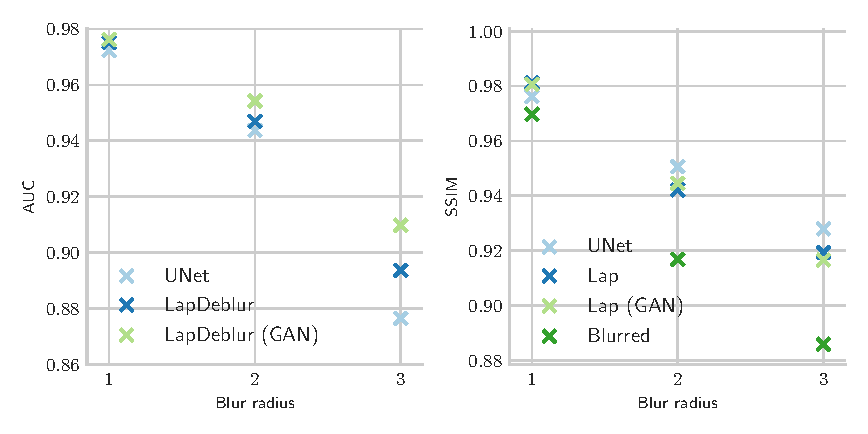
\includegraphics[]{deblur_complete_paper}
\caption{Measurements on Drive(Test).
  Blur radius vs.\ metric.\\
Segmentation on blurred images directly leads to an AUC of 0.96, 0.83 and 0.65 respectively.}
\label{fig:benchmark}
\end{figure}
% \todo{PSNR table}
\todo{Segmentation table: Frangi}
\todo{Evaluate speed}

\begin{figure}[htb]
\centering
\begin{subfigure}{0.45\textwidth}
\centering
    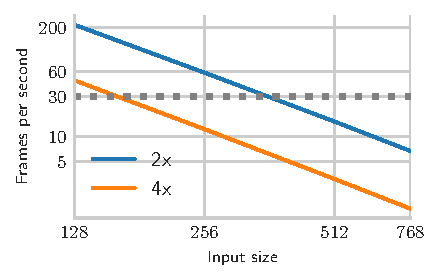
\includegraphics[]{time_upscaling_paper}
    \caption{Speed for upscaling}
\end{subfigure}\quad\qquad%
\begin{subfigure}{0.45\textwidth}
\centering
    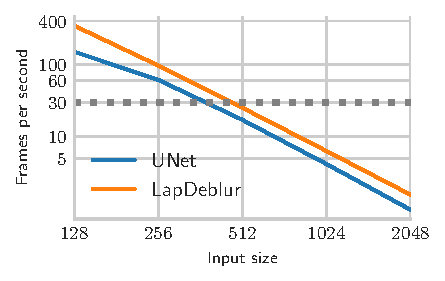
\includegraphics{time_denoising_paper}
    \caption{Speed for denoising}
\end{subfigure}
\caption{Frames per second vs.\ input image size.
Measured on a Titan X.}
\label{fig:benchmark}
\end{figure}

\section{Summary}
\todo{write summary}
% \begin{enumerate}
% \item We compare different loss functions and their suitability for medical image denoising.
% \item We present models that are able to reconstruct images detoriated by both mentioned downsampling operators in real-time.
% \item We evaluate the resulting algorithms on both diagnostic and intraoperative images and discuss their robustness against Blur.
%   This is combined with a discussion of the effectiveness of our transfer learning approach.
% \end{enumerate}

The presented models work well for diagnostic images.
They are efficient and result in both faithful and perceptual satisfying images.
While the individual loss functions result in good reconstructions, our chosen combination is clearly superior by all used metrics.
The adversarial loss leads to images that are more smooth but deviate from the data, sometimes introducing additional vessels or other artefacts.

The algorithms satisfy all our constraints:
% \begin{enumerate}
% \item All processing should happen in real time.
% \item It has to work with images of varying quality, level of zoom and different positions of surgical instruments.
% \item The anatomical structure, the position of surgical instruments, and the color have to be conserved.
% Both blood vessels and the border of the membrane should be at least as clearly visible as in the original images.
% This implies that we have to preserve the image edges.
% \end{enumerate}
\begin{itemize}
\item The algorithms work in real-time for small patch sizes.
  If a faster speed is desired our super-resolution network is also able to output $2\times$ resolved images.
\item The deblurring network is robust to different levels of blur.
  It is able to improve the segmentation results on all tested blur intensities.
\item All networks except the ones trained with adversarial loss retain the structure of blood vessels.
  They can thus be used for medical purposes.
\end{itemize}

\printbibliography
\end{document}